\documentclass{article}

\usepackage{tikz}
\usetikzlibrary{calc,positioning}

\pgfdeclarelayer{background}
\pgfsetlayers{background,main}

\begin{document}

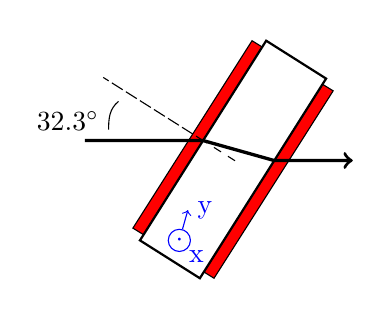
\begin{tikzpicture}
  % crystal
  \draw [thick,fill=white]
    (0,0) node [circle] (crystal1) {}
    -- ++(57.7:3)
      coordinate [pos=0.5] (laserin)
      node [pos=1,circle] (crystal2) {}
    -- ++(-32.3:0.9)
      node [circle] (crystal3) {}
    -- ++(237.7:3)
      node [circle] (crystal4) {}
    -- cycle
  ;
  % coating
  \begin{pgfonlayer}{background}
    \draw [fill=red]
      (crystal1.120)
      -- (crystal2.180)
      -- (crystal3.300)
      -- (crystal4.0)
      -- cycle
    ;
  \end{pgfonlayer}
  % normal
  \draw [dashed]
    (laserin)
    -- +(147.7:1.5)
      node [pos=0.75] (angledash) {}
    -- +(147.7:-0.5)
  ;
  % beam
  \draw [very thick, ->]
    ($(laserin) - (1.5,0)$)
    -- (laserin)
      node [pos=0.2] (anglebeam) {}
    -- ++(-15.7:0.936)
    -- ++(1,0)
  ;
  % input angle marker
  \draw
    (angledash)
    to [out=220,in=90] (anglebeam)
    node [above left] {$32.3^\circ$}
  ;
  %axes
  \node [draw,blue,circle,inner sep=1pt] 
    at (0.5,0) (axes) {$\cdot$}
  ;
  \draw [blue,->] 
    (axes)
      node [below right] {x}
    -- ++(74.3:0.4)
      node [right] {y}
  ;
\end{tikzpicture}

\end{document}

